\documentclass[14pt,fleqn]{extarticle}
\RequirePackage{prepwell}
\previewoff
\begin{document}

%text
Find the area of the region 
%
\[ \quad \lbrace (x,y): x^2+y^2\leq 4, x + y\geq 2 \rbrace \]

\newcard

\begin{center}
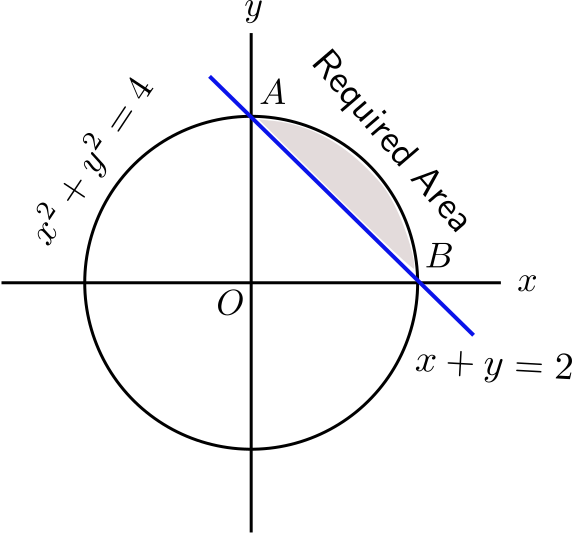
\includegraphics[scale=0.35]{img_right.svg}
\end{center}

\newcard

\begin{center}

\includegraphics[scale=0.35]{img_wrong.svg}
\end{center}

\newcard

We haven't been given a diagram showing which area to calculate\newline 

Instead we have been given the \underline{set of $(x,y)$} that make up the required area and some conditions that $(x,y)$ must satisfy 

\begin{center}
  \begin{tabular}{Nl}
  \toprule 
        \text{Condition} & Meaning \\
   \midrule 
     x^2 + y^2 \leq 4 &  On or inside the circle $x^2+y^2 = 4$ \\
    \midrule 
    x + y \geq 2 & Above the line $x+y = 2$ \\
    \bottomrule
  \end{tabular}
\end{center}

Only an $(x,y)$ in the shaded region below satisfies both the conditions 

\begin{center}
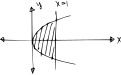
\includegraphics[scale=0.35]{right.svg}
\end{center}
%

\newcard

The required area $R$ will be given by 
\begin{align}
R &= \int_0^2 \sqrt{4-x^2}\cdot dx + \int_0^2 x\cdot dx - 2\int_0^2 dx
\end{align} 

\newcard

The required area $R$ will be given by 
\begin{align}
R &= \int_0^2 \sqrt{4-x^2}\cdot dx - \int_0^2 x\cdot dx + 2\int_0^2 dx
\end{align}

\newcard

%text
The circle \& the line intersect when 
%
\begin{align}
y^2 = \underbrace{4-x^2}_{\text{circle}} &= \underbrace{(2-x)^2}_{\text{line}}\\
\implies 4-x^2 = 4 + x^2 - 4x & \text{ or }  2x^2-4x = 0 \\
\implies 2x\cdot(x-2) &= 0 \text{ or } x = 0,2 
\end{align} 
%text

The required area, therefore, will be 
%
\begin{align}
R &= \underbrace{\int_0^2 \sqrt{4-x^2}\cdot dx}_{\text{under the circle}} 
- \underbrace{\int_0^2 (2-x)\cdot dx}_{\text{under the line}} \\
&= \int_0^2 \sqrt{4-x^2}\cdot dx + \int_0^2 x\cdot dx - 2\int_0^2 dx
\end{align}

\newcard

\[ R = \pi - 2\] 

\newcard

\[ R = \pi - 1\] 

\newcard

%
\begin{align}
R &= \int_0^2 \sqrt{4-x^2}\cdot dx + \int_0^2 x\cdot dx - 2\int_0^2 dx\\
&= \underbrace{\frac{1}{2}\cdot\left[ x\sqrt{4-x^2}+2^2\cdot\sin^{-1}\frac{x}{2}\right]_0^2}
_{\int\sqrt{a^2-x^2}dx = \frac{1}{2}\cdot\left[x\sqrt{a^2-x^2}+a^2\sin^{-1}\frac{x}{a}\right]}+\left[\frac{x^2}{2}\right]_0^2 - 2\left[ x\right]_0^2 \\
&= \frac{4}{2}\underbrace{\sin^{-1}\frac{2}{2}}_{=\frac\pi{2}} + \frac{4}{2} - 2\cdot 2 \\
&= 2\cdot\frac\pi{2} + 2 - 4 = \pi - 2
\end{align}

\end{document}
